\textbf{\underline{\large{4.1: Extrema and the Derivative Tests}}} \par

One of the most valuable aspects of calculus is that it allows us to find extreme values of functions. The ability to find maximum or minimum values of functions has wide-ranging applications. Every industry has uses for finding extremes, from optimizing profit and loss, to maximizing output of a chemical reaction, to minimizing surface areas of packages. This one tool of calculus eventually revolutionized the way the entire world approached every aspect of industry. It allowed people to solve formerly unsolvable problems. \par

\begin{tcolorbox}[objective]
    \begin{center}
        OBJECTIVES \\[11pt]
    \end{center}
    Find Critical Values and Extreme Values for Functions \\
    Use the 1\st and 2\nd Derivative Tests to Identify Maxima v.s. Minima
\end{tcolorbox}

But, before we begin, let's review some definitions from last year, which will be useful in this chapter as well as subsequent chapters. \par

\begin{tcolorbox}[definition]
    \begin{tabbing}
        \textit{Critical Value} $\rightarrow$ \= The $x$-coordinate of the extreme. 
    \end{tabbing} \vspace{11pt}
    \begin{tabbing}
        \textit{Maximum Value} $\rightarrow$ \= The $y$-coordinate of the high point. 
    \end{tabbing} \vspace{11pt}
    \begin{tabbing}
        \textit{Minimum Value} $\rightarrow$ \= The $y$-coordinate of the low point. 
    \end{tabbing} \vspace{11pt}
    \begin{tabbing}
        \textit{Relative Extremes} $\rightarrow$ \= The highest or lowest point in a given section of the curve. 
    \end{tabbing} \vspace{11pt}
    \begin{tabbing}
        \textit{Absolute Extremes} $\rightarrow$ \= The highest or lowest point of the whole curve. 
    \end{tabbing} \vspace{11pt}
    \begin{tabbing}
        \textit{Interval of Increasing} $\rightarrow$ \= The interval of $x$-values for which the curve is rising from left \\
        \> to right.
    \end{tabbing} \vspace{11pt}
    \begin{tabbing}
        \textit{Interval of Decreasing} $\rightarrow$ \= The interval of $x$-values for which the curve is dropping from \\
        \> left to right.
    \end{tabbing}
\end{tcolorbox}

\begin{center}
    \fbox{\fbox{\begin{minipage}{0.96 \textwidth}
        \vspace{11pt}
        Critical values of a function occur when: \par
        \vspace{11pt}
        \begin{center}
            \begin{tabular}{l}
                1) $\deriv = 0$ \\[11pt]
                2) $\deriv$ does not exist \\[11pt]
                3) the function reaches an endpoint of its domain
            \end{tabular}
        \end{center}
    \end{minipage}}}
\end{center}

It's also helpful to remember that a \textbf{critical value} is referring specifically to the value of the $x$, while the \textbf{extreme value} refers to the value of the $y$. \par
As we already know, the first derivative is what allows us to algebraically find extremes, and the First Derivative Test allows us to interpret critical values as maxima or minima. Since the first derivative of a function tells us when that function is increasing or decreasing, we can figure out if a critical value is associated with a maximum or minimum depending on the sign change of the derivative. Let's quickly refresh our memory on the First Derivative Test. \par

\begin{center}
    \fbox{\fbox{\begin{minipage}{0.96 \textwidth}
        \vspace{11pt}
        \begin{center}
            \textbf{The First Derivative Test}
        \end{center}
        \vspace{11pt}
        As the sign pattern of the first derivative is viewed left to right, the critical value represents a:
        \begin{center}
            \begin{tabular}{l}
                1) relative maximum if the sign changes from $+$ to $-$ \\[11pt]
                2) relative minimum if the sign changes from $-$ to $+$ \\[11pt]
                3) neither a relative max or min if the sign does not change
            \end{tabular}
        \end{center}
    \end{minipage}}}
\end{center}

\begin{tcolorbox}[example]
    \textbf{Ex 4.1.1: } Apply the First Derivative Test to the function $y = 5x^4 - 10x^2$.
\end{tcolorbox}
\begin{tcolorbox}[solution]
    \textbf{Sol 4.1.1: } \begin{align*}
        \deriv = 20x^3 - 20x &= 0 \\[11pt]
        20x\left(x^2 - 1\right) &= 0 \\[11pt]
        x &= -1, \, 0, \, 1
    \end{align*} 
    Now, let's make our sign pattern. \\
    \begin{center}
        \begin{tikzpicture}[baseline=(current bounding box.center)]
            \draw[<->, thick] (0,0) -- (8,0);

            \node at (2, -0.6) {$-1$};
            \node at (4, -0.6) {$0$};
            \node at (6, -0.6) {$1$};
            \node at (-0.5, -0.6) {$x$};

            \node at (1,0.5) {$-$};
            \node at (2,0.5) {$0$};
            \node at (3,0.5) {$+$};
            \node at (4,0.5) {$0$};
            \node at (5,0.5) {$-$};
            \node at (6,0.5) {$0$};
            \node at (7,0.5) {$+$};
            \node at (-0.5, 0.5) {$y'$};
        \end{tikzpicture}
    \end{center}
    So, there appear to be critical values at $x$ values of $-1, \, 0$, and $1$. By utilizing the First Derivative Test, we can see that we have a $\boxed{\text{minimum at } -1}$, a $\boxed{\text{maximum at } 0}$, and another $\boxed{\text{minimum at } 1}$.
\end{tcolorbox} \vspace{11pt}

\begin{tcolorbox}[example]
    \textbf{Ex 4.1.2: } Find the maximum values for the function $g(x) = \sqrt{x^3 - 9x}$.
\end{tcolorbox}
\begin{tcolorbox}[solution]
    \textbf{Sol 4.1.2: } For this question, we have to be careful! Because we are dealing with a square root, we will have domain restrictions. We can find such restrictions by starting with a sign pattern for $g(x)$. \\
    \begin{center}
        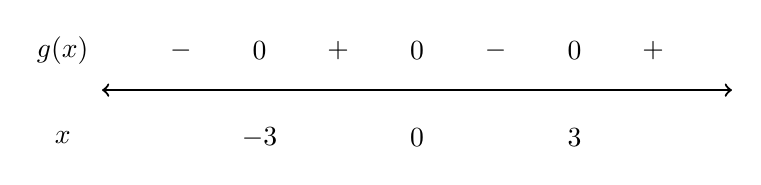
\begin{tikzpicture}[baseline=(current bounding box.center)]
            \draw[<->, thick] (0,0) -- (8,0);

            \node at (2, -0.6) {$-3$};
            \node at (4, -0.6) {$0$};
            \node at (6, -0.6) {$3$};
            \node at (-0.5, -0.6) {$x$};

            \node at (1,0.5) {$-$};
            \node at (2,0.5) {$0$};
            \node at (3,0.5) {$+$};
            \node at (4,0.5) {$0$};
            \node at (5,0.5) {$-$};
            \node at (6,0.5) {$0$};
            \node at (7,0.5) {$+$};
            \node at (-0.5, 0.5) {$g(x)$};
        \end{tikzpicture}
    \end{center}
    Now, since we know that the argument of a square root has to be positive, we know that our domain is when $x^3 - 9x \geq 0$. Therefore, based on our sign pattern, our domain is $x \in [-3, \, 0] \cup [3, \infty)$. \par
    \vspace{11pt}
    With that out the way, we can now take the first derivative and apply the First Derivate Test. \begin{align*}
        g'(x) &= \dfrac{3x^2 - 9}{2\sqrt{x^3 - 9x}} \\[11pt]
        g'(x) &= 0 \text{ when } 3x^2 - 9 = 0 \therefore x = \pm \sqrt{3} \\[11pt]
        g'(x) &= DNE \text{ when } x^3 - 9x = 0 \therefore x = \pm 3, \, 0
    \end{align*}
    Since $x = \sqrt{3}$ is not in the domain of the function, our critical values are at $x = \pm 3, \, 0, -\sqrt{3}$. Therefore, our sign pattern looks like: \\
    \begin{center}
        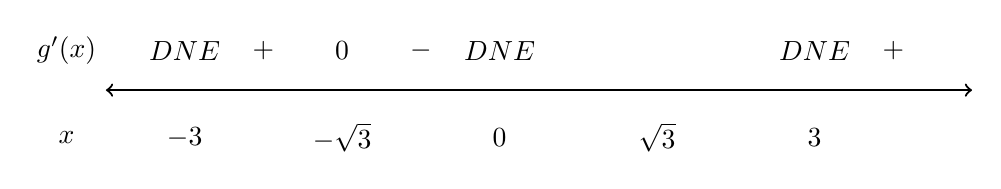
\begin{tikzpicture}[baseline=(current bounding box.center)]
            \draw[<->, thick] (0,0) -- (11,0);

            \node at (1, -0.6) {$-3$};
            \node at (3, -0.6) {$-\sqrt{3}$};
            \node at (5, -0.6) {$0$};
            \node at (7, -0.6) {$\sqrt{3}$};
            \node at (9, -0.6) {$3$};
            \node at (-0.5, -0.6) {$x$};

            \node at (1,0.5) {$DNE$};
            \node at (2,0.5) {$+$};
            \node at (3,0.5) {$0$};
            \node at (4,0.5) {$-$};
            \node at (5,0.5) {$DNE$};
            \node at (7,0.5) {};
            \node at (9,0.5) {$DNE$};
            \node at (10,0.5) {$+$};
            \node at (-0.5, 0.5) {$g'(x)$};
        \end{tikzpicture}
    \end{center}
    From our sign pattern, we can conclude that at $x = -\sqrt{3}$, we have a maximum value, and by substituting this value into the function, we find the maximum value is at $\boxed{y = 3.224}$.
\end{tcolorbox}

The First Derivative Test is not the only way to test whether critical values are associated with maximum or minimum values. If you recall, the second derivative can show us intervals of concavity. This is very useful because if we know that the curve is concave down at a critical value, it must be associated with a maximum. Similarly, if the curve is concave up, the critical value must be associated with a minimum value. \par

\begin{center}
    \fbox{\fbox{\begin{minipage}{0.96\textwidth}
        \vspace{11pt}
        \begin{center}
            \textbf{The Second Derivative Test}
        \end{center}
        \vspace{11pt}
        For a function $f$: 
        \vspace{11pt}
        \begin{center}
            1) If $f'(c) = 0$ and $f''(c) > 0$, then $f$ has a relative minimum at $c$ \\[11pt]
            2) If $f'(c) = 0$ and $f''(c) < 0$, then $f$ has a relative maximum at $c$ \\[11pt]
        \end{center}
    \end{minipage}}}
\end{center}

Now, we can revisit \textbf{Ex 1.5.7} part (c), which we previously could not do without the Second Derivative Test. \par

\begin{tcolorbox}[example]
    \textbf{Ex 4.1.3: } Consider the curve given by $x^2 + 4xy + y^2 = -12$. \\
    \begin{enumerate}[label=\hspace{11pt}(\alph*), align=left, leftmargin=*, labelsep=0.25em, start=3]
        \item Find the value(s) of $\deriv[2] \forcespace$ at the point(s) found in part (b). Does the curve have a local maximum, a local minimum, or neither at those points? Justify your answer.
    \end{enumerate} \vspace{11pt}
    \footnotesize{\textit{(Ex 1.5.7)}}
\end{tcolorbox} 
\begin{tcolorbox}[solution]
    \textbf{Sol 4.1.3: } What is really asked here is to apply the Second Derivative Test, because we cannot create a sign pattern for non-functions. The $y$ is not isolated in the equation. Recall that the two points we found in part (b) were $(-4, \, 2)$ and $(4, \, -2)$.\begin{align*}
        & \deriv[2] \begin{aligned}[t]
            & = \diff \left[\deriv = -\dfrac{x + 2y}{2x + y}\right] \\[11pt]
            & = \dfrac{(2x + y)\left(1 + 2\deriv\right) - (x + 2y)\left(2 + \deriv\right)}{(2x + y)^2} \\[11pt]
        \end{aligned} \\[11pt]
        & \deriv[2] \eval_{(-4, 2)} \begin{aligned}[t]
            & = \dfrac{(2(-4) + 2)\left(1 + 2(0)\right) - (-4 + 2(2))\left(2 + 0\right)}{(2(-4) + 2)^2} \\[11pt]
            & = \dfrac{6}{(-6)^2} > 0
        \end{aligned} \\[11pt]
        & \deriv[2] \eval_{(4, -2)} \begin{aligned}[t]
            & = \dfrac{(2(4) - 2)\left(1 + 2(0)\right) - (4 + 2(-2))\left(2 + 0\right)}{(2(4) + 2)^2} \\[11pt]
            & = \dfrac{6}{(-6)^2} < 0
        \end{aligned}
    \end{align*}
    $\boxed{(-4, 2) \text{ will be a minimum}}$ because the second derivative is positive. \\[11pt]
    $\boxed{(4, -2) \text{ will be a maximum}}$ because the second derivative is negative.
\end{tcolorbox} \vspace{11pt}

\begin{tcolorbox}[example]
    \textbf{Ex 4.1.4: } Use the Second Derivative Test to determine if the critical values of $g(t) = 27t - t^3$ are at a maximum or minimum value.
\end{tcolorbox} 
\begin{tcolorbox}[solution]
    \textbf{Sol 4.1.4: } \begin{align*}
        g'(t) = 27 - 3t^2 &= 0 \\[11pt]
        t &= \pm 3
    \end{align*}
    So, $-3$ and $3$ are critical values. Now, let's take a look at the second derivative of $g(t)$ at those values. \begin{align*}
        g''(t) &= -6t \\[11pt]
        g''(-3) &= -6(-3) = 18 \\[11pt]
        g''(3) &= -6(3) = -18
    \end{align*}
    Finally, we can apply the Second Derivative Test. Since $g'(-3) = 0$ and $g''(-3) > 0$, we can determine that $\boxed{t = -3 \text{ is a minimum}}$. Similarly, since $g'(3) = 0$ and $g''(3) < 0$, we can determine that $\boxed{t = 3 \text{ is a maximum}}$. Note that the numerical value of the second derivative is irrelevant --- only the sign matters.
\end{tcolorbox} \vspace{11pt}

\begin{tcolorbox}[example]
    \textbf{Ex 4.1.4: } Determine if the critical values of $y = \left(3 - x^2\right)e^x$ are at a maximum or a minimum value. 
\end{tcolorbox}
\begin{tcolorbox}[solution]
    \textbf{Sol 4.1.4: } First, let's find the critical values. \begin{align*}
        \deriv = \left(3 - x^2\right)e^x + e^x(-2x) &= 0 \\[11pt]
        -e^x\left(x^2 + 2x - 3\right) &= 0 \\[11pt]
        -e^x(x + 3)(x - 1) &= 0
    \end{align*}
\end{tcolorbox}